\documentclass[a4paper,11pt,singlespacing]{article}

\usepackage{setspace}
\usepackage[utf8]{inputenc}
\usepackage[T1]{fontenc}
\usepackage{graphicx}
\usepackage{color}
\usepackage{hyperref}
\usepackage{listings,xcolor}

\renewcommand{\figurename}{Abbildung}

\graphicspath{ {./images/} }

\title{Projektskizze: WLAN-AP mit regelmäßigem PSK-Tausch und QR-Code Anmeldung}
\date{\today}

\begin{document}
	\setlength{\parindent}{0ex}
	\maketitle
	
	\section{Motivation}
	Der Hauptgrund für dieses Projekt war der umständliche Prozess der Anmeldung von Gästen im WLAN mit einem sicheren pre-shared Key. Dieser Key sollte aufgrund der Sicherheit lang und kryptisch gewählt sein. Somit muss man ihn bei jeder Anmeldung neu heraussuchen und eintippen. \\ \\
	Der Vorgang den Key manuell zu ändern ist zeitaufwendig und unnötig. Für die Sicherheit unserer Daten wird auf Produkte von Drittanbietern verzichtet. Hierfür soll mit diesem Projekt eine eigenständige Lösung mit Fokus auf einfacher Bedienung und komfortabler Sicherheit gemacht werden. 
	
	\section{Problem}
	Der pre-shared Key eines WLAN-Netzwerkes wird in den meisten Netzwerken einmal oder gar nicht geändert. Dadurch können Gäste dauerhaften Zugang zum Netzwerk behalten, obwohl das nicht erwünscht ist.  \\ \\ 
	Dies hat zur Folge, dass sich sobald einmal das Passwort geknackt oder bewusst/unbewusst weitergegeben wurde, jeder mit dem Access-Point verbinden kann. Regelmäßiges Wechseln des Keys führt jedoch zu unangenehmen Mehraufwand, den sehr viele Nutzer nicht eingehen wollen. Die Folge sind auf Dauer ungewollte Endgeräte im eigenen Netzwerk.
	
	\section{Lösungsansätze}
	Ein Lösungsansatz stellt ein sich automatisch oder auf Tastendruck ändernder pre-shared Key dar. Der Key wird jeden Montag morgen um 03:00 Uhr automatisch durch einen Cron-Job gewechselt. Der Taster kann zusätzlich betätigt werden, falls das Passwort sofort geändert werden soll. \\ 
	Der Key wird so gewählt,dass er nicht in dem Zeitraum geknackt werden kann bis ein neuer Key erzeugt wird. Mit diesem neu generierten Key können sich Endgeräte anmelden und kommunizieren. Hiermit wird das Problem der ungewollten Nutzern gelöst, denn diese können sich sobald der Key gewechselt hat, nicht mehr im Netz anmelden. Der Key wird an einem Display in zwei verschiedenen Varianten angezeigt:
	\begin{itemize}
		\item Klartext für Endgeräte ohne Kamera z.B. Laptops
		\item QR-Code zum Scannen für z.B Smartphones
	\end{itemize}

	Es wurde sich für einen QR-Code anstatt eines RFID/NFC Transponder entschieden, da hier die Möglichkeit des Abgreifens des Keys nicht besteht. In Abbildung  \ref{aufbau} ist der Aufbau des Lösungsansatzes graphisch dargestellt.

	\begin{figure}[ht]
		\centering
		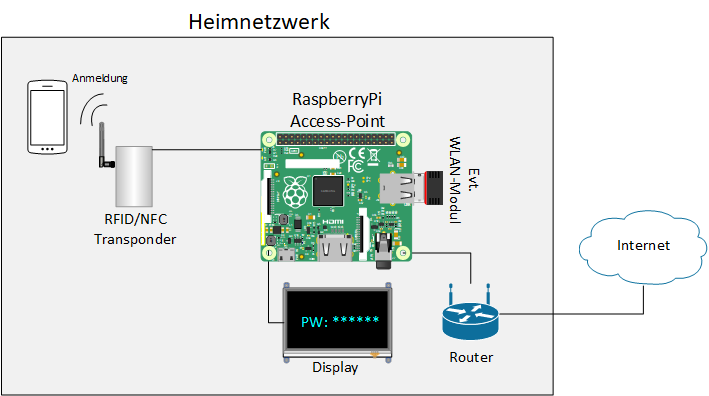
\includegraphics[scale=0.6]{skizze}
			\caption{Aufbau des Gastnetzes}
			\label{aufbau}
	\end{figure}

	
	\section{Anforderungsanalyse}

		\subsection{Hardware}
		Für dieses Projekt wird ein Raspberry Pi 3 B+ benötigt. Grund hierfür ist der HDMI Anschlusses, der aus komfort Gründen für den Display benutzt werden soll. Zudem hat dieses Modell ausreichend Leistung, ein integriertes WLAN-Modul und alle nötigen Anschlüsse:
		\begin{itemize}
			\item 2.4GHz and 5GHz IEEE 802.11.b/g/n/ac wireless LAN
			\item Extended 40-pin GPIO header
			\item Full-size HDMI
			\item Micro SD port für das Laden des Betriebsystems und zur Speicherung der Daten
			\item 5V/2.5A DC power input
			\item Ethernet Port
		\end{itemize}
		Zusätzlich wird eine Mikro-SD Karte zum Laden des Betriebsystems und zur Speicherung der Daten benötigt \\ \\
		Das Display, welches verwendet wird, muss eine ausreichende Auflösung für die Darstellung des QR - Codes besitzen. Deshalb können keine der kleineren und billigeren LCD Anzeigen verwendet werden. Außerdem muss diese noch an den Raspberry Pi in Form von HDMI angeschlossen werden, da die Pins für mögliche Schalter/Umschalter verwendet werden können.
		
		\subsection{Software}
		Um den Raspberry Pi als Access-Point verwenden zu können, müssen zusätzliche Pakete installiert und eine Netzwerkkonfiguration vorgenommen werden. Darunter fällt das Einstellen von DHCP und DNS für die Clients, sowie das erzeugen des Keys. \\ \\
		Der Key hat 10 Zeichen und verwendet werden dürfen die Zeichen 95. Der verwendete Algorithmus ist . Angenommen ein Rechner schafft 2 Billionen Keys pro Sekunde würde er 346 Tage benötigen, um alle Keys zu testen. Auch wenn er zur Hälfte der Zeit den richtigen Key findet, sind wir auf der sicheren Seite. 
		\begin{eqnarray}
			(95^{10})/2000000000000 =  29936846.961918945312\\
			29936846.961918945312 / 60 /60 /24 \approx 346
		\end{eqnarray}
		Als Skriptsprache empfiehlt sich Python, da es sehr viele Libraries gibt, die einiges an Arbeit abnehmen. Zudem kann man mit Python auf einfache Kommandos des Betriebsystems zugreifen. Für die QR-Code Generierung eignen sich die Libraries qrcode und PyQRCode. Für die Generierung eines Keys wird das Programm pwgen benutzt.\\ \\
		Zum Schluss muss der neu generierte Key den Alten ersetzen.
		
		\subsection{Tests}
		Zu Testzwecken werden unterschiedliche Smartphones (Android/iOS) und Notebooks (Windows/Linux/macOS) benutzt. So soll Sichergestellt werden, dass mögliche Probleme aufgrund von Diskrepanzen zwischen den Betriebssystemen bzw. Hardware erkannt werden.
	
	\section{Priorisierung}
	
	Das wichtigste zu Beginn ist, dass die Hardware aufeinander abgestimmt wird. Bedeutet, alle Teile passen zusammen und können angeschlossen werden.
	Danach muss die Konfiguration des Raspberry Pi zum Access-Point erfolgen. Sobald dies funktioniert kann das Generieren des pre-shared Keys und dessen Austausch stattfinden. Folglich wird die Ausgabe des Keys am Bildschirm realisiert. Danach kann dies, um das Generieren des QR-Codes und dessen Ausgabe erweitert werden.\\
	Wenn diese Punkte voll funktional umgesetzt werden konnten, kann sich um einen automatischen oder manuellen Job (bei Tastendruck) zum Generieren und Austauschen des Keys gekümmert werden.
		
		\subsection{Zielgruppe}
		Das Projekt ist für Haushalte geeignet, welche ein sicheres Gästenetz gewährleisten möchten. Es kann außerdem von Firmen genutzt werden, die für Besucher und Mitarbeiter WLAN zur Verfügung stellen möchten und diese nicht für immer in ihrem Netz haben möchten. 
		
		\subsection{Funktionen}
		Im Folgenden werden die verschiedenen Funktionen definiert und kategorisiert.
			\subsubsection{Grundlegende Funktionen}
			\begin{itemize}
				\item Funktionerender Access-Point
				\item Automatisches Wechseln des Keys
				\item Ausgabe als Text
				\item Ausgabe als QR-Code
			\end{itemize}
		
			\subsubsection{Optionale Funktionen}
			\begin{itemize}
				\item Anbindung eines Tasters zum manuellen Tausch des Keys 
				\item Energiesparen durch an- und abschalten des Displays
				\item Skript zum Automatisieren der Konfiguration
			\end{itemize}


Hardware aufeinander abstimmen 
Konfiguration des Raspberry Pi zum Access Point
Generieren des Keys
Austausch des Keys zur Anmeldung
Ausgabe des Keys in Textform auf das Display
Generieren des QR-Codes
Ausgabe des QR-Codes auf das Display
\end{document}
